\documentclass[letterpaper,12pt]{article}

\usepackage{threeparttable}
\usepackage{geometry}
\geometry{letterpaper,tmargin=1in,bmargin=1in,lmargin=1.25in,rmargin=1.25in}
\usepackage[format=hang,font=normalsize,labelfont=bf]{caption}
\usepackage{amsmath}
\usepackage{mathrsfs}
\usepackage{multirow}
\usepackage{array}
\usepackage{delarray}
\usepackage{listings}
\usepackage{amssymb}
\usepackage{amsthm}
\usepackage{lscape}
\usepackage{natbib}
\usepackage{setspace}
\usepackage{float,color}
\usepackage[pdftex]{graphicx}
\usepackage{pdfsync}
\usepackage{verbatim}
\usepackage{placeins}
\usepackage{geometry}
\usepackage{pdflscape}
\synctex=1
\usepackage{hyperref}
\hypersetup{colorlinks,linkcolor=red,urlcolor=blue,citecolor=red}
\usepackage{bm}


\theoremstyle{definition}
\newtheorem{theorem}{Theorem}
\newtheorem{acknowledgement}[theorem]{Acknowledgement}
\newtheorem{algorithm}[theorem]{Algorithm}
\newtheorem{axiom}[theorem]{Axiom}
\newtheorem{case}[theorem]{Case}
\newtheorem{claim}[theorem]{Claim}
\newtheorem{conclusion}[theorem]{Conclusion}
\newtheorem{condition}[theorem]{Condition}
\newtheorem{conjecture}[theorem]{Conjecture}
\newtheorem{corollary}[theorem]{Corollary}
\newtheorem{criterion}[theorem]{Criterion}
\newtheorem{definition}{Definition} % Number definitions on their own
\newtheorem{derivation}{Derivation} % Number derivations on their own
\newtheorem{example}[theorem]{Example}
\newtheorem{exercise}[theorem]{Exercise}
\newtheorem{lemma}[theorem]{Lemma}
\newtheorem{notation}[theorem]{Notation}
\newtheorem{problem}[theorem]{Problem}
\newtheorem{proposition}{Proposition} % Number propositions on their own
\newtheorem{remark}[theorem]{Remark}
\newtheorem{solution}[theorem]{Solution}
\newtheorem{summary}[theorem]{Summary}
\bibliographystyle{aer}
\newcommand\ve{\varepsilon}
\renewcommand\theenumi{\roman{enumi}}
\newcommand\norm[1]{\left\lVert#1\right\rVert}

\begin{document}

\title{581 HW 1,2}
\author{Chris Rytting}
\maketitle

\subsection*{1.1}

First set of parameters:\\
\\
$\tilde{k}_t$:
\begin{align*}
\\\text{mean} &= 2.44142065	
\\\text{standard deviation} &= 0.016548655
\\\text{coefficient of variation}&=147.529857	
\\\text{relative coefficient of variation}&=34.70249165
\\\text{correlation with Y}&=0.008751021
\\\text{correlation with A}&=0.067324833
\\\text{autocorrelation}&=0.977701483
\end{align*}
For $\tilde{y}_t$ 

\begin{align*}
\\\text{mean} &= 16.62386659
\\\text{standard deviation} &= 3.910324347
\\\text{coefficient of variation}&=4.251275627
\\\text{relative coefficient of variation}&=1
\\\text{correlation with Y}&=1
\\\text{correlation with A}&=-0.007854036
\\\text{autocorrelation}&=0.023820669
\end{align*}
\\
$\tilde{c}_t$
\begin{align*}
\\\text{mean} &= 15.79267326
\\\text{standard deviation} &=3.71480813
\\\text{coefficient of variation}&=4.251275627
\\\text{relative coefficient of variation}&=1
\\\text{correlation with Y}&=1
\\\text{correlation with A}&=-0.007854036
\\\text{autocorrelation}&=0.023820669
\end{align*}
\\
$\tilde{i}_t$
\begin{align*}
\\\text{mean} &= 0.83119333
\\\text{standard deviation} &= 0.195516217
\\\text{coefficient of variation}&=4.251275627
\\\text{relative coefficient of variation}&=1
\\\text{correlation with Y}&=1
\\\text{correlation with A}&=-0.007854036
\\\text{autocorrelation}&=0.023820669
\end{align*}
$\tilde{A}_t$
\begin{align*}
\\\text{mean} &= 1.58956E+19
\\\text{standard deviation} &= 8.99959E+19
\\\text{coefficient of variation}&=0.176625269
\\\text{relative coefficient of variation}&=0.041546417
\\\text{correlation with Y}&=-0.007854036
\\\text{correlation with A}&=1
\\\text{autocorrelation}&=0.996937289
\end{align*}
$log(\tilde{k}_t)$
\begin{align*}
\\\text{mean} &= 0.387632637
\\\text{standard deviation} &= 0.002943609
\\\text{coefficient of variation}&=131.6862025
\\\text{relative coefficient of variation}&=11.68364577
\\\text{correlation with Y}&=0.005119208
\\\text{correlation with A}&=0.069949226
\\\text{autocorrelation}&=0.977701483
\end{align*}
.\\
$log(\tilde{y}_t)$
\begin{align*}
\\\text{mean} &= 1.20806748
\\\text{standard deviation} &= 0.107183837
\\\text{coefficient of variation}&=11.27098554
\\\text{relative coefficient of variation}&=1
\\\text{correlation with Y}&=1
\\\text{correlation with A}&=-0.002328091
\\\text{autocorrelation}&=0.024272717
\end{align*}
$log(\tilde{C}_t)$
\begin{align*}
\\\text{mean} &= 1.185791085
\\\text{standard deviation} &= 0.107183837
\\\text{coefficient of variation}&=11.06315202
\\\text{relative coefficient of variation}&=0.981560306
\\\text{correlation with Y}&=1
\\\text{correlation with A}&=-0.002328091
\\\text{autocorrelation}&=0.024272717
\end{align*}
$log(\tilde{I}_t)$
\begin{align*}
\\\text{mean} &= -0.092962515
\\\text{standard deviation} &= 0.107183837
\\\text{coefficient of variation}&=-0.867318412
\\\text{relative coefficient of variation}&=-0.076951426
\\\text{correlation with Y}&=1
\\\text{correlation with A}&=-0.002328091
\\\text{autocorrelation}&=0.024272717
\end{align*}
$\tilde{Z}_t$
\begin{align*}
\\\text{mean} &= -0.000227542
\\\text{standard deviation} &= 0.077752194
\\\text{coefficient of variation}&=	-0.002926504
\\\text{relative coefficient of variation}&=-0.000259649
\\\text{correlation with Y}&=0.991863887
\\\text{correlation with A}&=-0.001159019
\\\text{autocorrelation}&=0.018696135
\end{align*}
For the second set of parameters:\\
$\tilde{k}_t$
\begin{align*}
\\\text{mean} &= 19.33021123
\\\text{standard deviation} &= 0.149250979
\\\text{coefficient of variation}&=129.5148037
\\\text{relative coefficient of variation}&=30.47115415
\\\text{correlation with Y}&=0.038584394
\\\text{correlation with A}&=-0.044818267
\\\text{autocorrelation}&=0.982903312
\end{align*}
$\tilde{y}_t$
\begin{align*}
\\\text{mean} &= 32.90138658
\\\text{standard deviation} &= 7.740761623
\\\text{coefficient of variation}&=4.250406896
\\\text{relative coefficient of variation}&=
\\\text{correlation with Y}&=
\\\text{correlation with A}&=-0.029745081
\\\text{autocorrelation}&=0.025466048
\end{align*}
\\
$\tilde{c}_t$
\begin{align*}
\\\text{mean} &= 26.32110927
\\\text{standard deviation} &= 6.192609298
\\\text{coefficient of variation}&=4.250406896
\\\text{relative coefficient of variation}&=1
\\\text{correlation with Y}&=1
\\\text{correlation with A}&=-0.029745081
\\\text{autocorrelation}&=0.025466048
\end{align*}
\\
$\tilde{i}_t$
\begin{align*}
\\\text{mean} &= 6.580277316
\\\text{standard deviation} &= 1.548152325
\\\text{coefficient of variation}&=4.250406896
\\\text{relative coefficient of variation}&=1
\\\text{correlation with Y}&=1
\\\text{correlation with A}&=-0.029745081
\\\text{autocorrelation}&=0.025466048
\end{align*}
$\tilde{A}_t$
\begin{align*}
\\\text{mean} &= 6.62065E+19
\\\text{standard deviation} &= 2.14821E+20
\\\text{coefficient of variation}&=0.308193504
\\\text{relative coefficient of variation}&=0.072509176
\\\text{correlation with Y}&=-0.029745081
\end{align*}
$log(\tilde{k}_t)$
\begin{align*}
\\\text{mean} &= 1.286636314
\\\text{standard deviation} &= 0.003312455
\\\text{coefficient of variation}&=388.4238386
\\\text{relative coefficient of variation}&=27.63552714
\\\text{correlation with Y}&=0.034335448
\\\text{correlation with A}&=-0.170332691
\\\text{autocorrelation}&=0.982366333
\end{align*}
$log(\tilde{y}_t)$

\begin{align*}
\\\text{mean} &= 1.506063174
\\\text{standard deviation} &=	0.108410611
\\\text{coefficient of variation}&=	13.89221185
\\\text{relative coefficient of variation}&=1
\\\text{correlation with Y}&=1
\\\text{correlation with A}&=	0.010024524
\\\text{autocorrelation}&=	0.023028172
\end{align*}
$log(\tilde{C}_t)$
\begin{align*}
\\\text{mean} &= 1.409153161
\\\text{standard deviation} &= 0.108410611
\\\text{coefficient of variation}&=12.99829554
\\\text{relative coefficient of variation}&=0.935653421
\\\text{correlation with Y}&=1
\\\text{correlation with A}&=0.010024524
\\\text{autocorrelation}&=0.023028172
\end{align*}
$log(\tilde{I}_t)$
\begin{align*}
\\\text{mean} &= 0.806622141
\\\text{standard deviation} &= 0.107129336
\\\text{coefficient of variation}&=7.529423524
\\\text{relative coefficient of variation}&=0.535750763
\\\text{correlation with Y}&=1
\\\text{correlation with A}&=-0.016170752
\\\text{autocorrelation}&=0.032461931
\end{align*}
$\tilde{Z}_t$
\begin{align*}
\\\text{mean} &= 0.000381011
\\\text{standard deviation} &= 0.077803028
\\\text{coefficient of variation}&=0.004897117
\\\text{relative coefficient of variation}&=0.000348451
\\\text{correlation with Y}&=0.991578612
\\\text{correlation with A}&=-0.01440627
\\\text{autocorrelation}&=0.030289601
\end{align*}

For the third set of parameters:\\
$\tilde{k}_t$
\begin{align*}
\\\text{mean} &= 2.44154615
\\\text{standard deviation} &= 0.018281284
\\\text{coefficient of variation}&=133.5544155
\\\text{relative coefficient of variation}&=31.46094187
\\\text{correlation with Y}&=0.030572945
\\\text{correlation with A}&=0.009737369
\\\text{autocorrelation}&=0.981720227
\end{align*}
$\tilde{y}_t$
\begin{align*}
\\\text{mean} &= 16.62615487
\\\text{standard deviation} &= 3.91656457
\\\text{coefficient of variation}&=4.245086369
\\\text{relative coefficient of variation}&=1
\\\text{correlation with Y}&=1
\\\text{correlation with A}&=-0.017171241
\\\text{autocorrelation}&=0.032961885
\end{align*}
\\
$\tilde{c}_t$
\begin{align*}
\\\text{mean} &= 15.79484713
\\\text{standard deviation} &= 	3.720736342
\\\text{coefficient of variation}&=	4.245086369
\\\text{relative coefficient of variation}&=1
\\\text{correlation with Y}&=1
\\\text{correlation with A}&=-0.017171241
\\\text{autocorrelation}&=	0.032961885
\end{align*}
\\
$\tilde{i}_t$
\begin{align*}
\\\text{mean} &= 0.831307744
\\\text{standard deviation} &= 0.195828229
\\\text{coefficient of variation}&=4.245086369
\\\text{relative coefficient of variation}&=1
\\\text{correlation with Y}&=1
\\\text{correlation with A}&=-0.017171241
\\\text{autocorrelation}&=0.032961885
\end{align*}
$\tilde{A}_t$
\begin{align*}
\\\text{mean} &= 3.99127E+19
\\\text{standard deviation} &=	1.82093E+20
\\\text{coefficient of variation}&=0.219188954
\\\text{relative coefficient of variation}&= 0.051633568
\\\text{correlation with Y}&=-0.017171241
\\\text{correlation with A}&=1	
\\\text{autocorrelation}&=0.996454884
\end{align*}
$log(\tilde{k}_t)$
\begin{align*}
\\\text{mean} &= 0.387652754
\\\text{standard deviation} &= 0.003253728
\\\text{coefficient of variation}&=119.1410971
\\\text{relative coefficient of variation}&=10.60446978
\\\text{correlation with Y}&=0.031172048
\\\text{correlation with A}&=0.028851351
\\\text{autocorrelation}&=0.981720227
\end{align*}
$log(\tilde{y}_t)$
\begin{align*}
\\\text{mean} &= 1.208067305
\\\text{standard deviation} &= 0.107527239
\\\text{coefficient of variation}&=11.2349886
\\\text{relative coefficient of variation}&=1
\\\text{correlation with Y}&=1
\\\text{correlation with A}&=-0.004345455
\\\text{autocorrelation}&=0.031840109
\end{align*}
$log(\tilde{C}_t)$
\begin{align*}
\\\text{mean} &= 1.18579091
\\\text{standard deviation} &= 0.107527239
\\\text{coefficient of variation}&=11.02781881
\\\text{relative coefficient of variation}&=0.981560303
\\\text{correlation with Y}&=1
\\\text{correlation with A}&=-0.004345455
\\\text{autocorrelation}&=0.031840109
\end{align*}
$log(\tilde{I}_t)$
\begin{align*}
\\\text{mean} &= -0.092086473
\\\text{standard deviation} &= 0.107459799
\\\text{coefficient of variation}&=-0.856938823
\\\text{relative coefficient of variation}&=-0.07617103
\\\text{correlation with Y}&=1
\\\text{correlation with A}&=0.015610874
\\\text{autocorrelation}&=0.034508809
\end{align*}
$\tilde{Z}_t$
\begin{align*}
\\\text{mean} &= 0.000561621
\\\text{standard deviation} &= 0.077553116
\\\text{coefficient of variation}&=0.007241762
\\\text{relative coefficient of variation}&=0.000637963
\\\text{correlation with Y}&=0.992130811
\\\text{correlation with A}&=0.010751721
\\\text{autocorrelation}&=0.020834155
\end{align*}

\subsection*{1.2}


\begin{figure}[H]
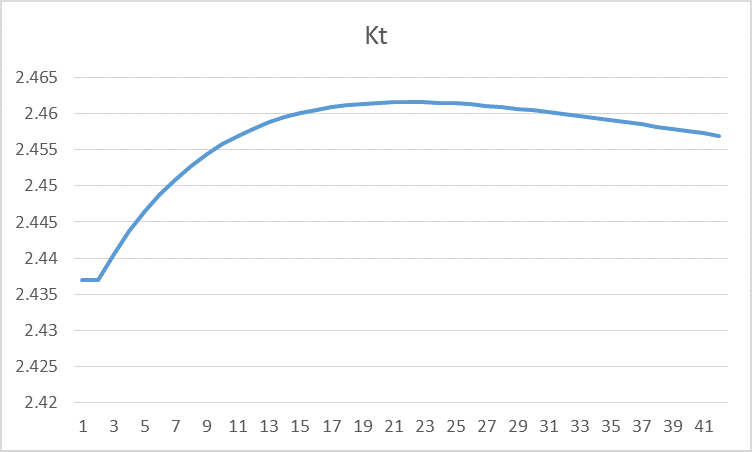
\includegraphics[scale=.50]{12a.png}
\end{figure}
\begin{figure}[H]
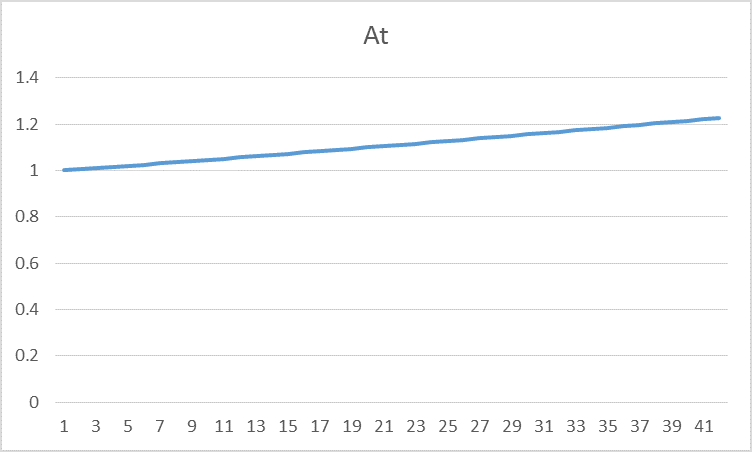
\includegraphics[scale=.50]{12b.png}
\end{figure}
\begin{figure}[H]
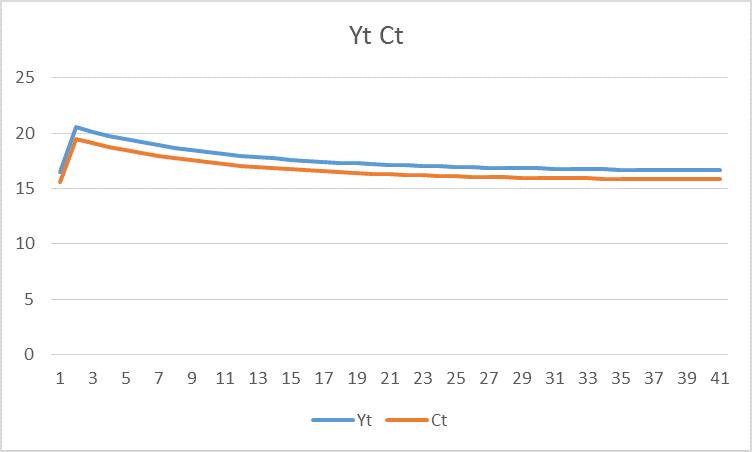
\includegraphics[scale=.50]{12c.png}
\end{figure}
\begin{figure}[H]
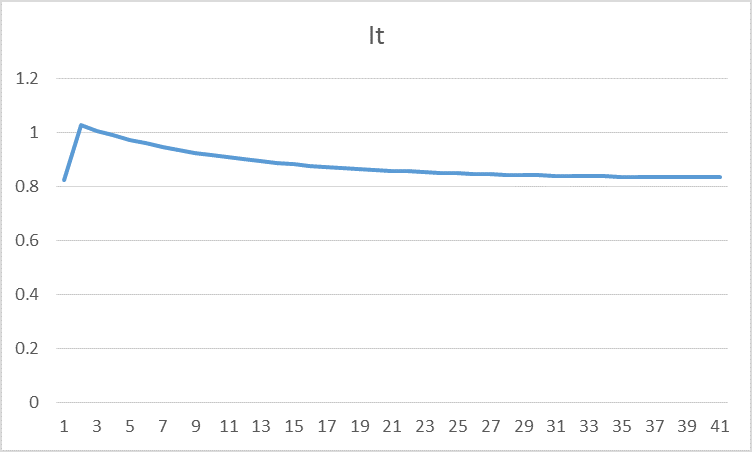
\includegraphics[scale=.50]{12d.png}
\end{figure}
\begin{figure}[H]
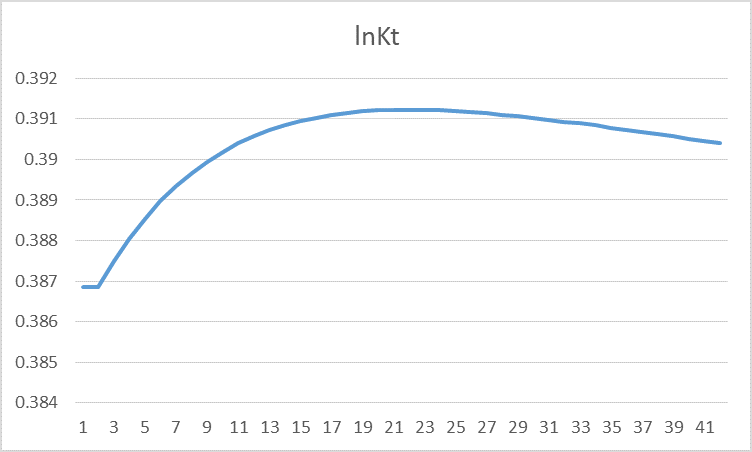
\includegraphics[scale=.50]{12e.png}
\end{figure}
\begin{figure}[H]
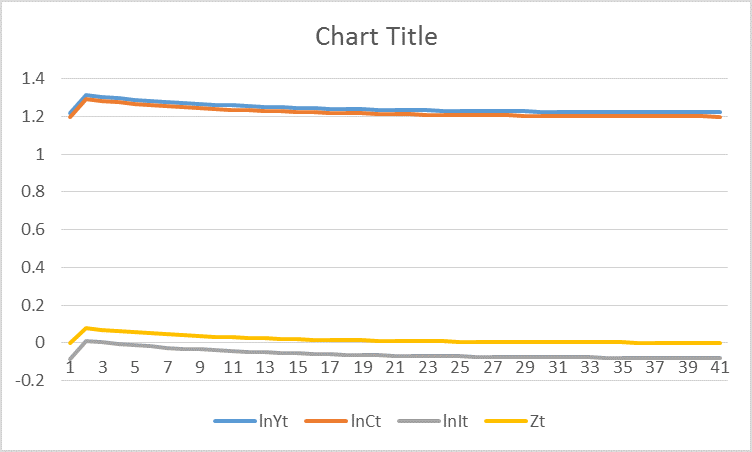
\includegraphics[scale=.50]{12f.png}
\end{figure}

\subsection*{1.3}


For the first set of paramaters:
$\tilde{k}_t$
\begin{align*}
\\\text{mean} &= 22.33412442
\\\text{standard deviation} &= 2.436367142
\\\text{coefficient of variation}&=0.003270556
\\\text{relative coefficient of variation}&=744.9396976
\\\text{correlation with Y}&=22.2741009
\\\text{correlation with A}&=0.999083849
\\\text{autocorrelation}&=0.120164945
\end{align*}
$\tilde{y}_t$
\begin{align*}
\\\text{mean} &= 16.44194142
\\\text{standard deviation} &= 	0.491622964
\\\text{coefficient of variation}&=33.44420952
\\\text{relative coefficient of variation}&=1
\\\text{correlation with Y}&=1
\\\text{correlation with A}&=0.811330798
\\\text{autocorrelation}&=0.999862829
\end{align*}
\\
$\tilde{c}_t$
\begin{align*}
\\\text{mean} &= 15.61984435
\\\text{standard deviation} &= 	0.467041816
\\\text{coefficient of variation}&=33.44420952
\\\text{relative coefficient of variation}&=1
\\\text{correlation with Y}&=1
\\\text{correlation with A}&=0.811330798
\\\text{autocorrelation}&=0.999862829
\end{align*}
\\
$\tilde{i}_t$
\begin{align*}
\\\text{mean} &= 0.822097071
\\\text{standard deviation} &= 	0.024581148
\\\text{coefficient of variation}&=33.44420952
\\\text{relative coefficient of variation}&=1
\\\text{correlation with Y}&=1
\\\text{correlation with A}&=0.811330798
\\\text{autocorrelation}&=0.999862829
\end{align*}
$\tilde{A}_t$
\begin{align*}
\\\text{mean} &= 0.999745803
\\\text{standard deviation} &= 	0.001699629
\\\text{coefficient of variation}&=588.2142476
\\\text{relative coefficient of variation}&=17.58792497
\\\text{correlation with Y}&=0.811330798
\\\text{correlation with A}&=1
\\\text{autocorrelation}&=0.989321611
\end{align*}
$log(\tilde{k}_t)$
\begin{align*}
\\\text{mean} &= 10.30626613
\\\text{standard deviation} &= 	6.886540103
\\\text{coefficient of variation}&=1.496581154
\\\text{relative coefficient of variation}&=0.000718038
\\\text{correlation with Y}&=0.12033207
\\\text{correlation with A}&=0.097343628
\\\text{autocorrelation}&=0.999987972
\end{align*}
$log(\tilde{y}_t)$
\begin{align*}
\\\text{mean} &= 1.216082417
\\\text{standard deviation} &= 	0.000583459
\\\text{coefficient of variation}&=2084.265232
\\\text{relative coefficient of variation}&=1
\\\text{correlation with Y}&=1
\\\text{correlation with A}&=0.81132256
\\\text{autocorrelation}&=0.999862841
\end{align*}
$log(\tilde{C}_t)$
	2046.085324,	0.981681838,	1,	0.81132256,	0.999862841.\\
\begin{align*}
\\\text{mean} &= 1.193806022	0.000583459
\\\text{standard deviation} &= 
\\\text{coefficient of variation}&=
\\\text{relative coefficient of variation}&=
\\\text{correlation with Y}&=
\\\text{correlation with A}&=
\\\text{autocorrelation}&=
\end{align*}
$log(\tilde{I}_t)$
\begin{align*}
\\\text{mean} &= -0.084947579	
\\\text{standard deviation} &= 	0.000583459
\\\text{coefficient of variation}&=-145.5931623
\\\text{relative coefficient of variation}&=-0.069853472
\\\text{correlation with Y}&=1
\\\text{correlation with A}&=0.81132256
\\\text{autocorrelation}&=0.999862841
\end{align*}
$\tilde{Z}_t$
\begin{align*}
\\\text{mean} &= 0
\\\text{standard deviation} &= 0
\\\text{coefficient of variation}&=0
\\\text{relative coefficient of variation}&=0
\\\text{correlation with Y}&=0
\\\text{correlation with A}&=0
\\\text{autocorrelation}&=0
\end{align*}

\begin{figure}[H]
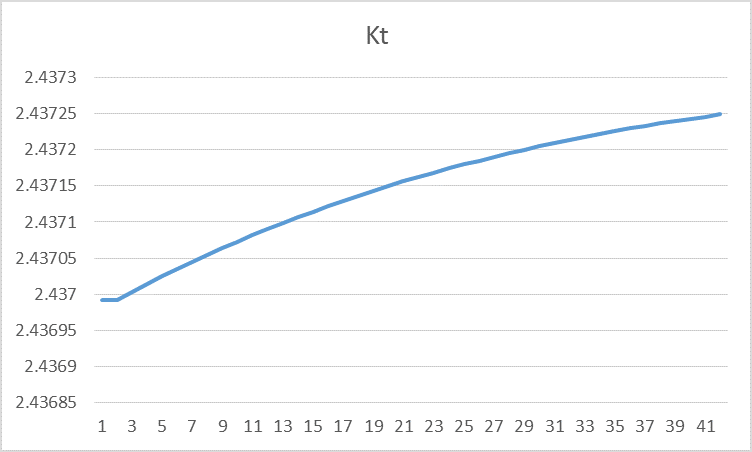
\includegraphics[scale=.50]{13a.png}
\end{figure}
\begin{figure}[H]
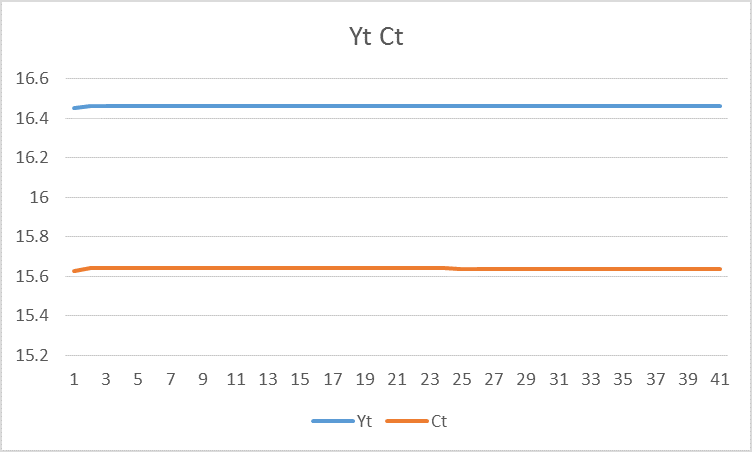
\includegraphics[scale=.50]{13b.png}
\end{figure}
\begin{figure}[H]
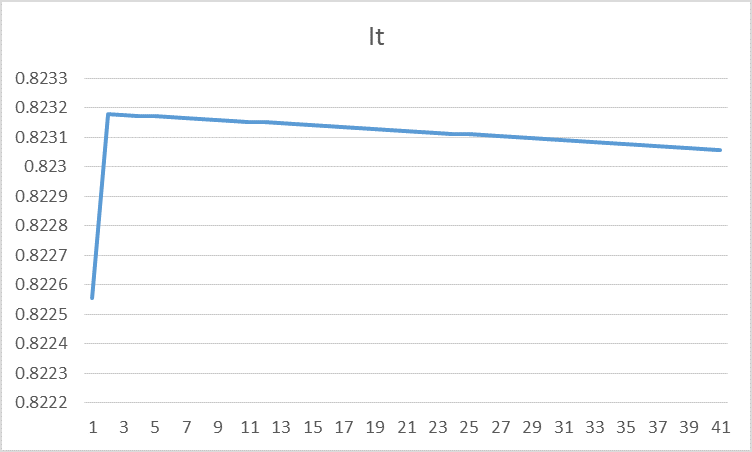
\includegraphics[scale=.50]{13c.png}
\end{figure}
\begin{figure}[H]
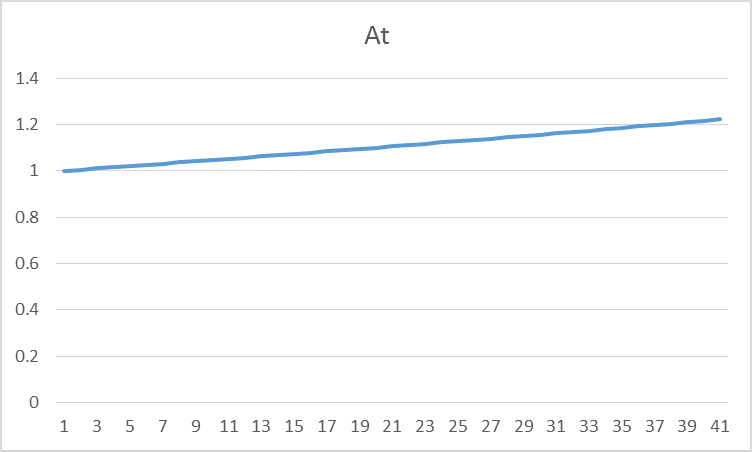
\includegraphics[scale=.50]{13d.png}
\end{figure}
\begin{figure}[H]
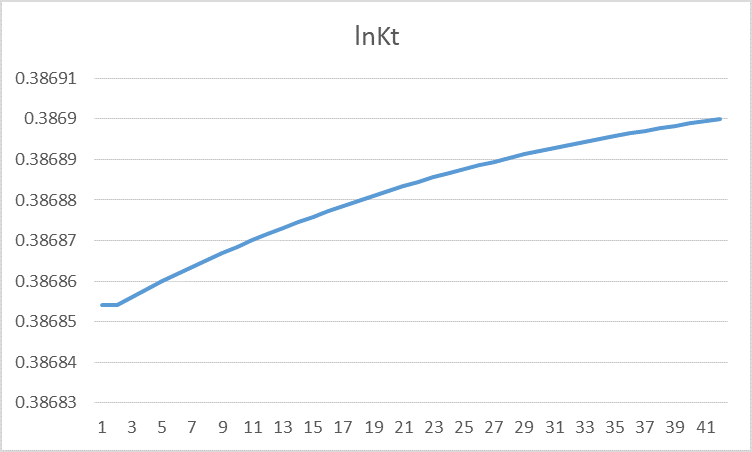
\includegraphics[scale=.50]{13e.png}
\end{figure}
\begin{figure}[H]
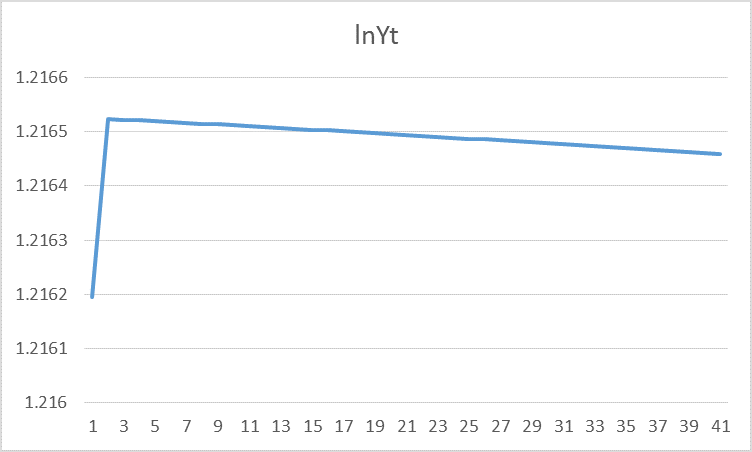
\includegraphics[scale=.50]{13f.png}
\end{figure}
\begin{figure}[H]
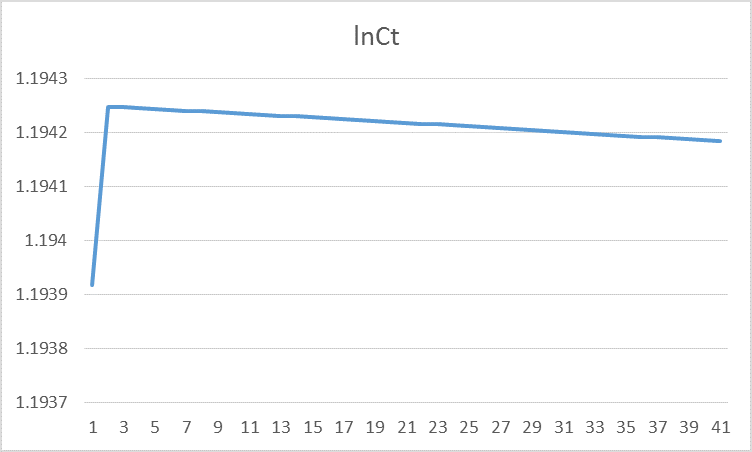
\includegraphics[scale=.50]{13g.png}
\end{figure}
\begin{figure}[H]
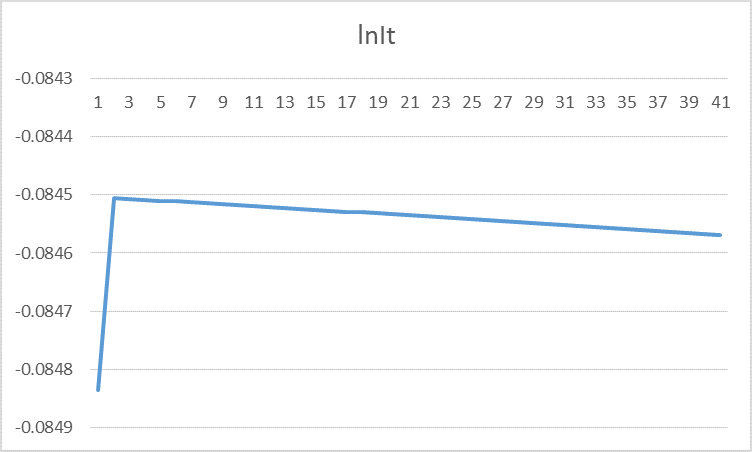
\includegraphics[scale=.50]{13h.png}
\end{figure}
\begin{figure}[H]
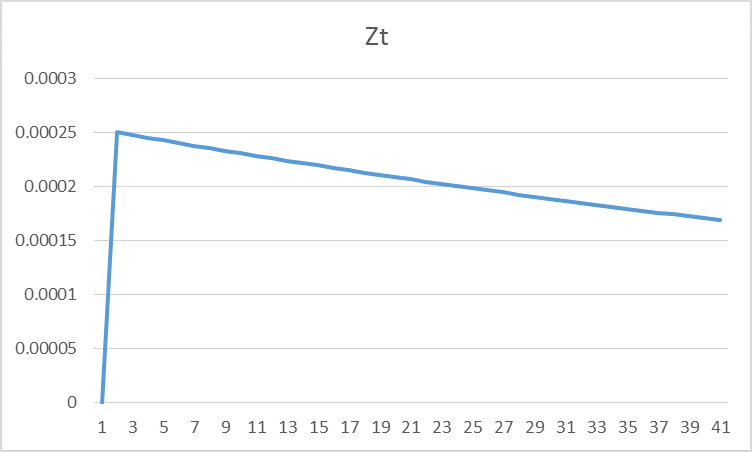
\includegraphics[scale=.50]{13i.png}
\end{figure}

For the second set of parameters:
$\tilde{k}_t$
\begin{align*}
\\\text{mean} &= 2.444678672
\\\text{standard deviation} &= 	0.020320086
\\\text{coefficient of variation}&=120.3084803
\\\text{relative coefficient of variation}&=28.79617487
\\\text{correlation with Y}&=0.045494757
\\\text{correlation with A}&=-0.112648907
\\\text{autocorrelation}&=0.984864362
\end{align*}
$\tilde{y}_t$
\begin{align*}
\\\text{mean} &= 16.73062081
\\\text{standard deviation} &= 	4.004521389
\\\text{coefficient of variation}&=4.177932687
\\\text{relative coefficient of variation}&=1
\\\text{correlation with Y}&=1
\\\text{correlation with A}&=0.023766636
\\\text{autocorrelation}&=0.044093365
\end{align*}
\\
$\tilde{c}_t$
\begin{align*}
\\\text{mean} &= 15.89408977
\\\text{standard deviation} &= 	3.804295319
\\\text{coefficient of variation}&=4.177932687
\\\text{relative coefficient of variation}&=1
\\\text{correlation with Y}&=1
\\\text{correlation with A}&=0.023766636
\\\text{autocorrelation}&=0.044093365
\end{align*}
\\
$\tilde{i}_t$
\begin{align*}
\\\text{mean} &= .83653104
\\\text{standard deviation} &= 	0.200226069
\\\text{coefficient of variation}&=4.177932687
\\\text{relative coefficient of variation}&=1
\\\text{correlation with Y}&=1
\\\text{correlation with A}&=0.023766636
\\\text{autocorrelation}&=0.044093365
\end{align*}
$\tilde{A}_t$
\begin{align*}
\\\text{mean} &= 0.999579122
\\\text{standard deviation} &= 	0.001868439
\\\text{coefficient of variation}&=534.9807613
\\\text{relative coefficient of variation}&=128.0491576
\\\text{correlation with Y}&=0.023766636
\\\text{correlation with A}&=1
\\\text{autocorrelation}&=0.990940538
\end{align*}
$log(\tilde{k}_t)$
\begin{align*}
\\\text{mean} &= 15.07415464
\\\text{standard deviation} &= 	8.296185049
\\\text{coefficient of variation}&=1.816998361
\\\text{relative coefficient of variation}&=0.161859889
\\\text{correlation with Y}&=-0.013069733
\\\text{correlation with A}&=-0.214748505
\\\text{autocorrelation}&=0.999991542
\end{align*}
$log(\tilde{y}_t)$
\begin{align*}
\\\text{mean} &= 1.210794062
\\\text{standard deviation} &= 	0.107858651
\\\text{coefficient of variation}&=11.22574823
\\\text{relative coefficient of variation}&=1
\\\text{correlation with Y}&=1
\\\text{correlation with A}&=0.022987192
\\\text{autocorrelation}&=0.045019853
\end{align*}
$log(\tilde{C}_t)$
\begin{align*}
\\\text{mean} &= 1.188517667	
\\\text{standard deviation} &= 0.107858651
\\\text{coefficient of variation}&=11.01921501
\\\text{relative coefficient of variation}&=0.98160183
\\\text{correlation with Y}&=1
\\\text{correlation with A}&=0.022987192
\\\text{autocorrelation}&=0.045019853
\end{align*}
$log(\tilde{I}_t)$
\begin{align*}
\\\text{mean} &= -0.090235934
\\\text{standard deviation} &= 	0.107858651
\\\text{coefficient of variation}&=-0.836612851
\\\text{relative coefficient of variation}&=-0.074526244
\\\text{correlation with Y}&=1
\\\text{correlation with A}&=0.022987192
\\\text{autocorrelation}&=0.045019853
\end{align*}
$\tilde{Z}_t$
\begin{align*}
\\\text{mean} &= 0.001499222	
\\\text{standard deviation} &=  0.078560334
\\\text{coefficient of variation}&=0.019083703
\\\text{relative coefficient of variation}&=0.001699479
\\\text{correlation with Y}&=0.991588202
\\\text{correlation with A}&=-0.011609685
\\\text{autocorrelation}&=0.037249566
\end{align*}






\subsection*{2.1}
\[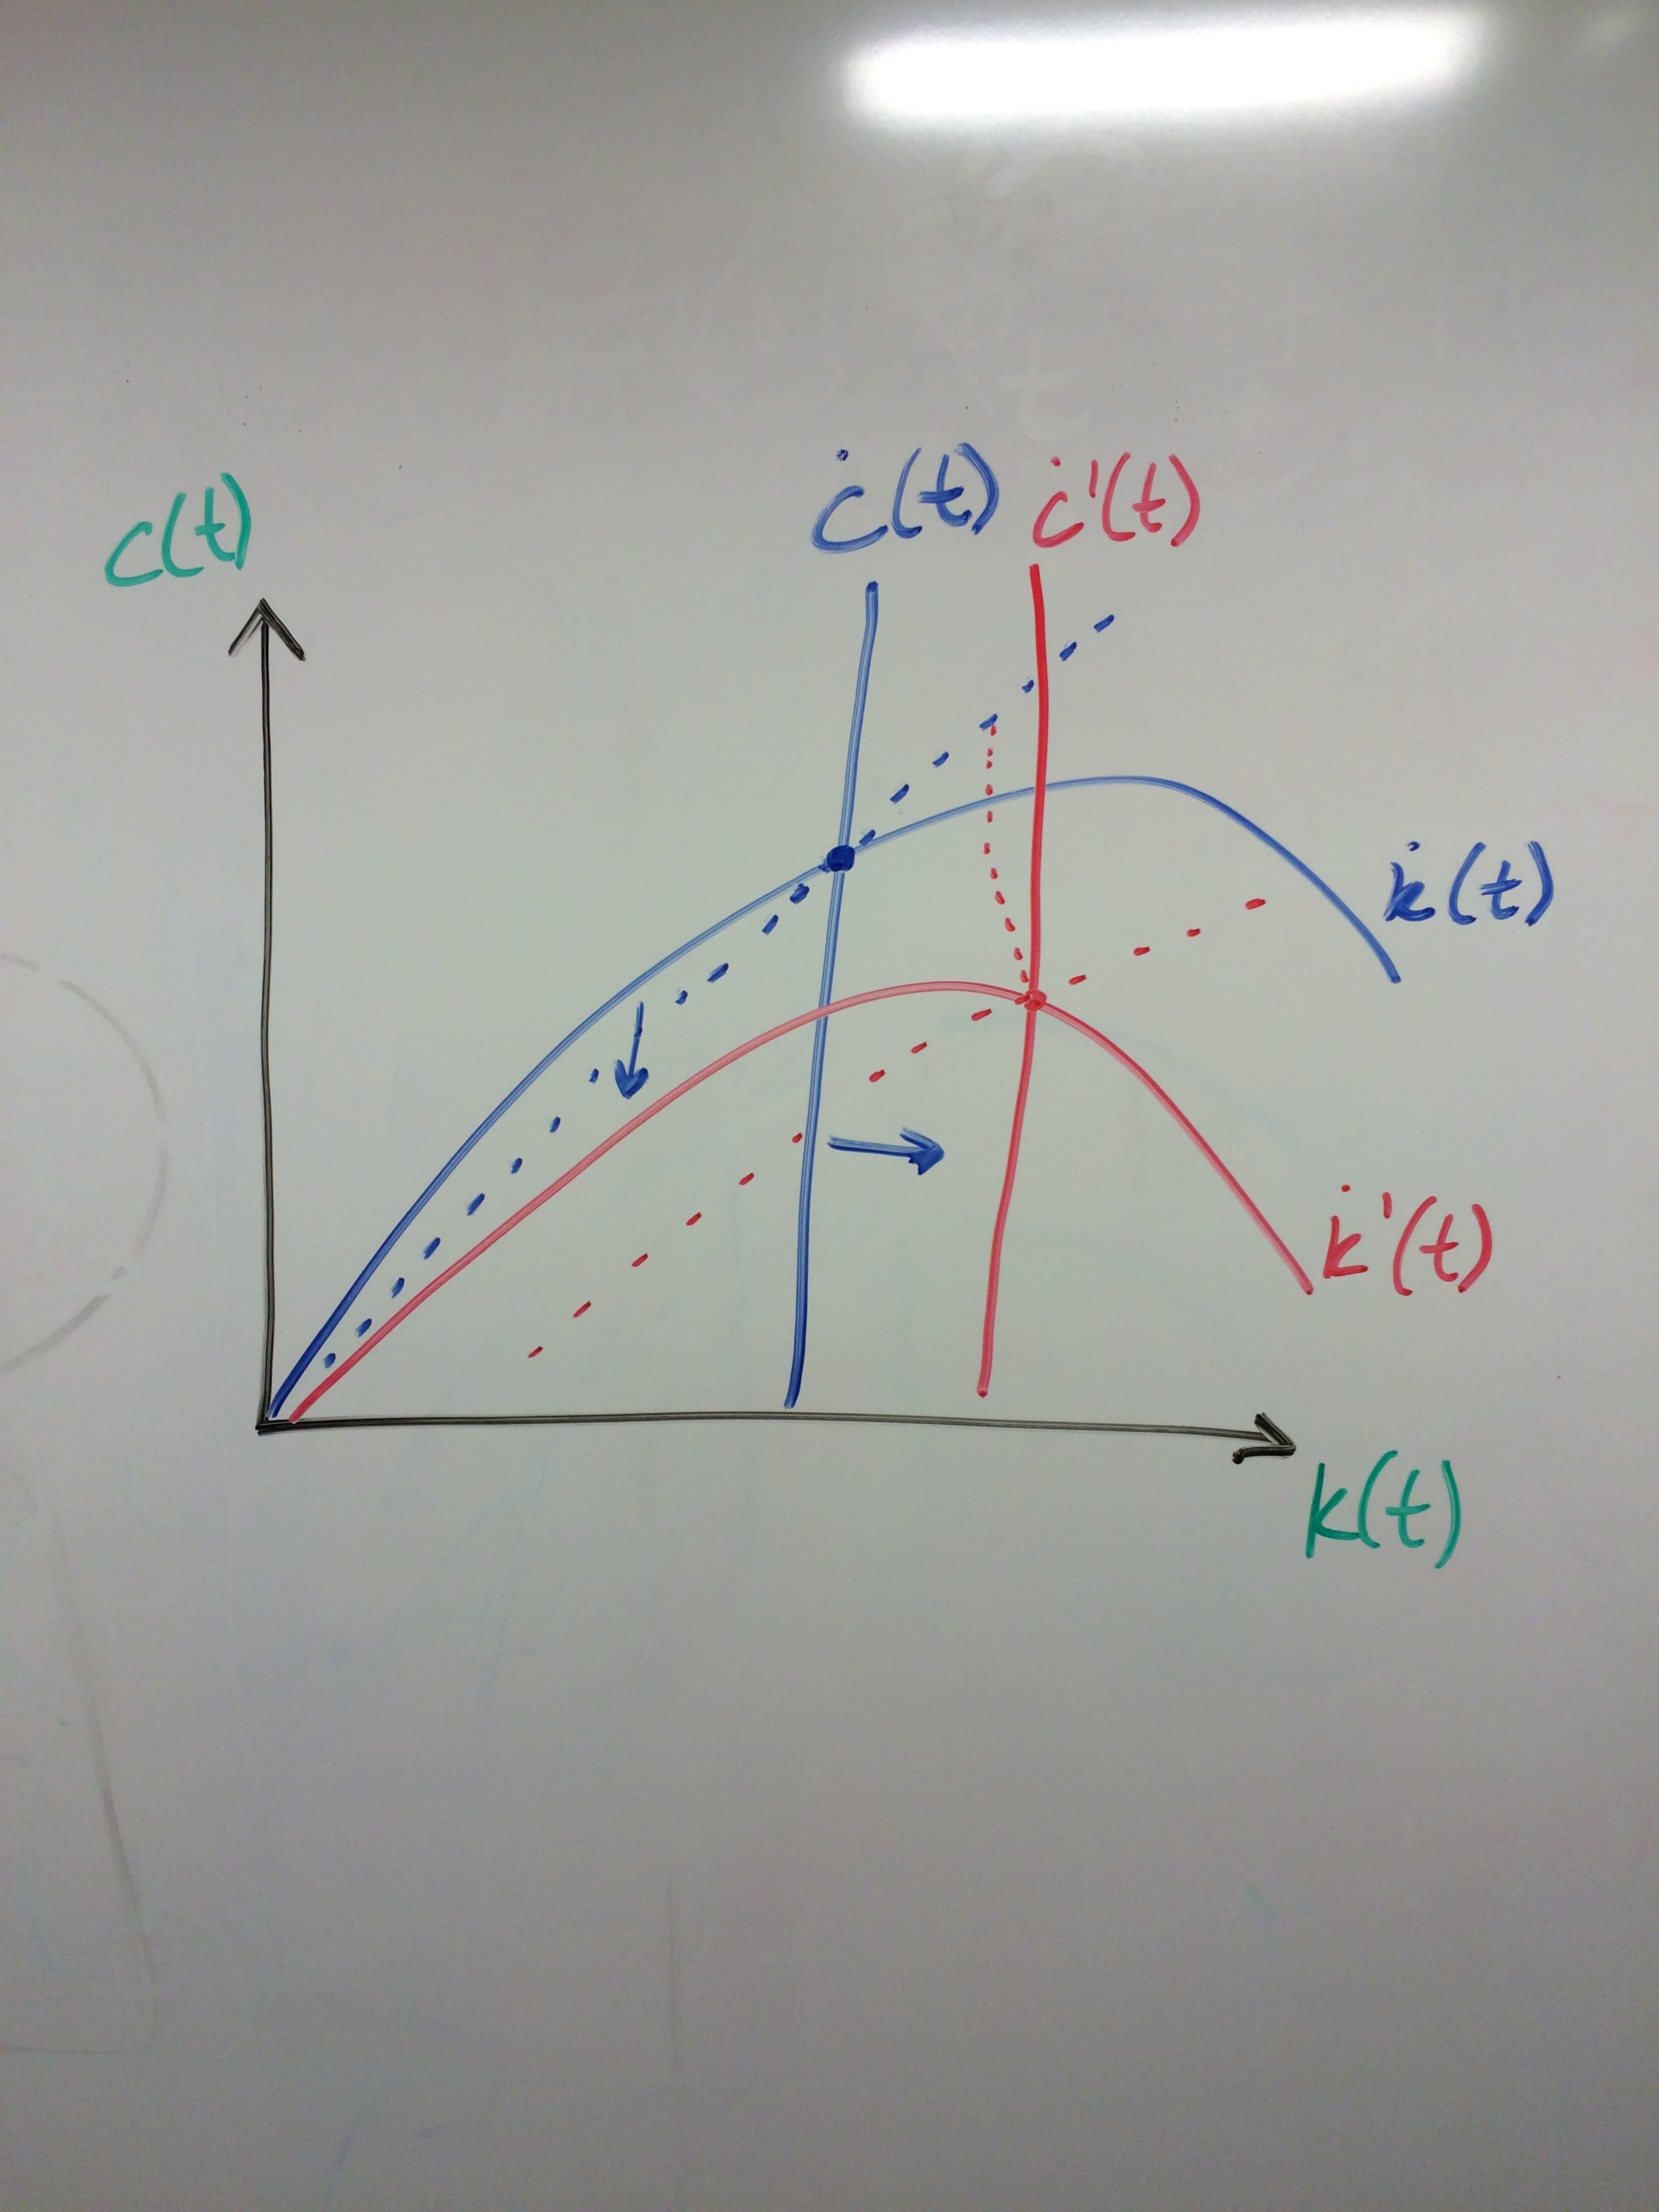
\includegraphics[scale = .05]{saddlegraph.jpg}\]
With an increase in $a$, consumption will increase immediately, then after date $S$ decrease to lower than previous levels before the equilibrium shifts to the new saddle point.
\subsection*{2.2}
With first parameter values, and shock of $.7$
\[\bar k = 25.5152058604\]
\[\bar y =  2.91235086459 \]
\[\bar c = 2.20996329086 \]
\[\bar r = 0.037666785468 \]
\[\bar w = 1.95127507927\]
\[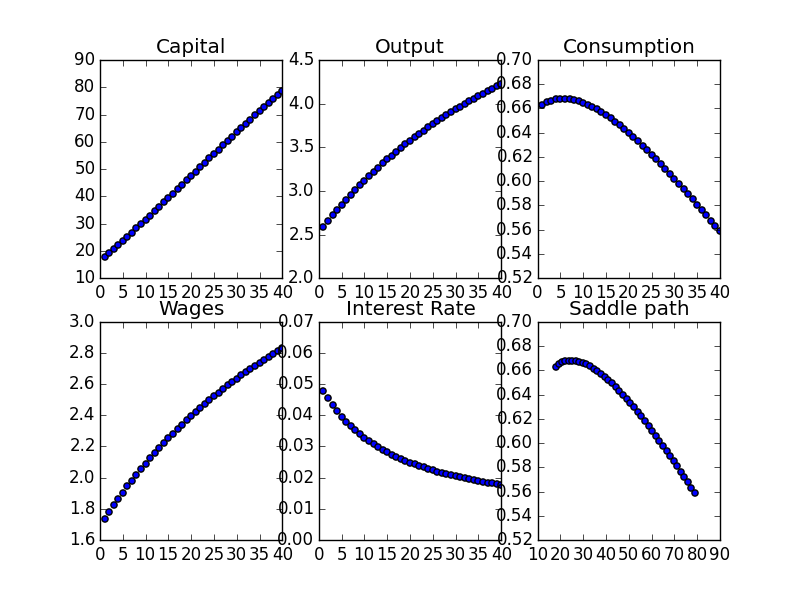
\includegraphics[scale = .5]{fig1.png}\]

With first parameter values, and shock of $1.5$
\[\bar k = 25.5152058604\]
\[\bar y =  2.91235086459 \]
\[\bar c = 2.20996329086 \]
\[\bar r = 0.037666785468 \]
\[\bar w = 1.95127507927\]
\[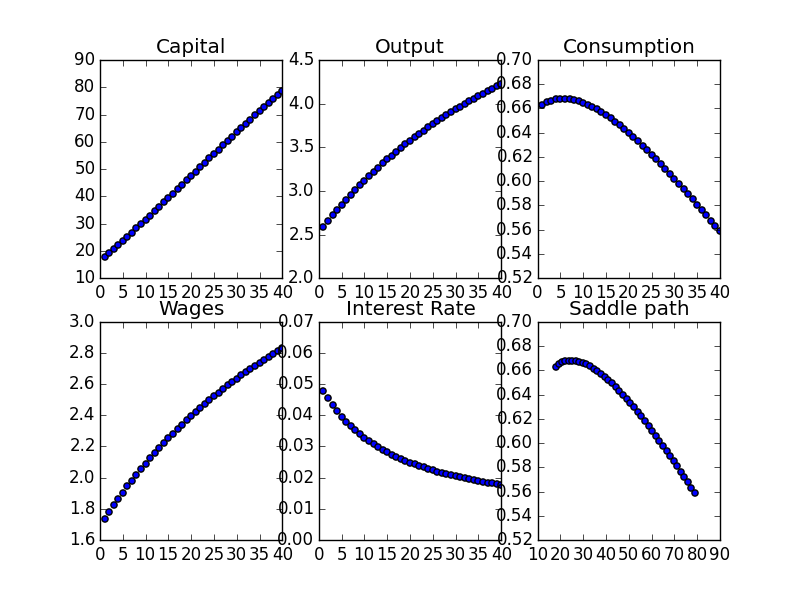
\includegraphics[scale = .5]{fig2.png}\]

With second parameter values, and shock of $.7$
\[\bar k = 35.7240923352\]
\[\bar y =  3.25444695343 \]
\[\bar c = 2.27102715755 \]
\[\bar r = 0.0300628350346 \]
\[\bar w = 2.1804794588\]
\[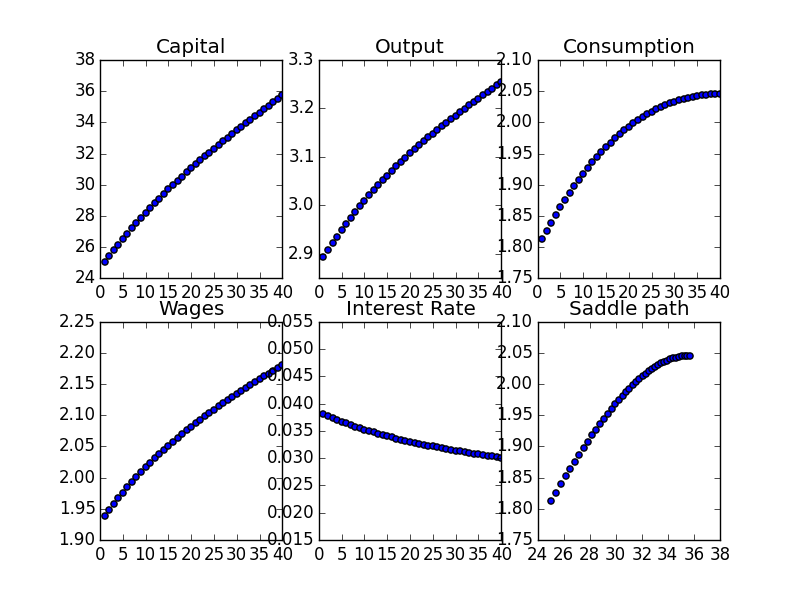
\includegraphics[scale = .5]{fig3.png}\]
   
With second parameter values, and shock of $1.5$
\[\bar k = 35.7240923352\]
\[\bar y =  3.25444695343 \]
\[\bar c = 2.27102715755 \]
\[\bar r = 0.0300628350346 \]
\[\bar w = 2.1804794588\]
\[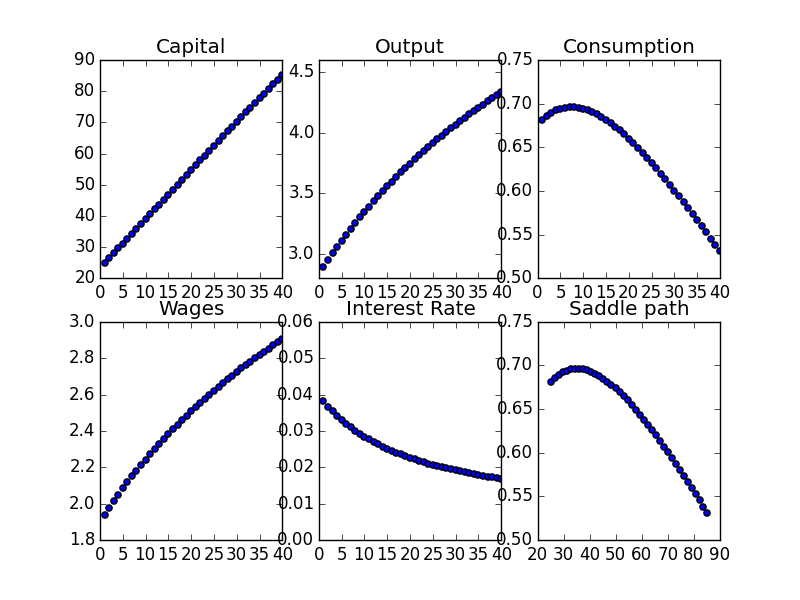
\includegraphics[scale = .5]{fig4.png}\]

With third parameter values, and shock of $.7$
\[\bar k = 7.45813055462\]
\[\bar y =  1.94074239883 \]
\[\bar c = 1.73543352327 \]
\[\bar r = 0.0858720542533 \]
\[\bar w = 1.30029740722\]
\[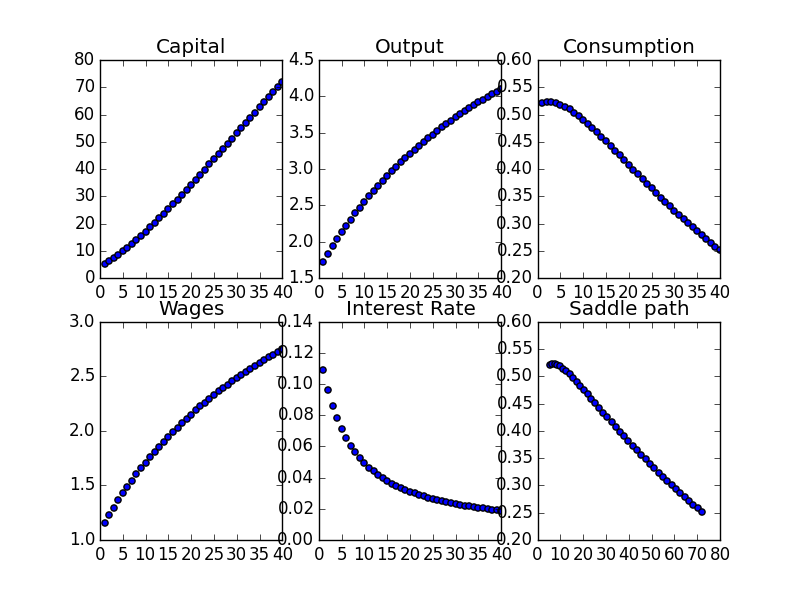
\includegraphics[scale = .5]{fig5.png}\]
   
With third parameter values, and shock of $1.5$
\[\bar k = 7.45813055462\]
\[\bar y =  1.94074239883 \]
\[\bar c = 1.73543352327 \]
\[\bar r = 0.0858720542533 \]
\[\bar w = 1.30029740722\]
\[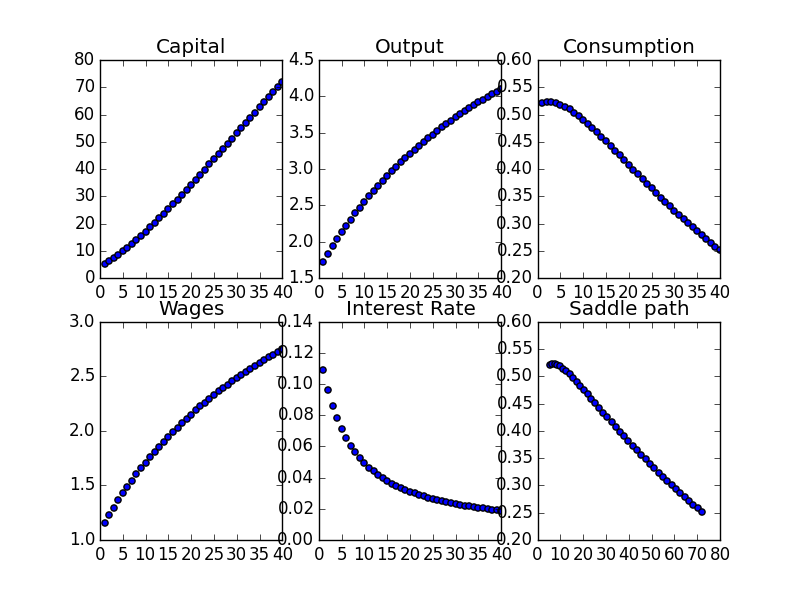
\includegraphics[scale = .5]{fig6.png}\]



\end{document}
